\section{Durchführung}
\label{sec:Durchfuehrung}
\subsection{Aufbau}
Für den Druckbereich von $p\leq 1$bar wird folgende Apperatur verwendet:
\begin{figure}[H]
    \centering
    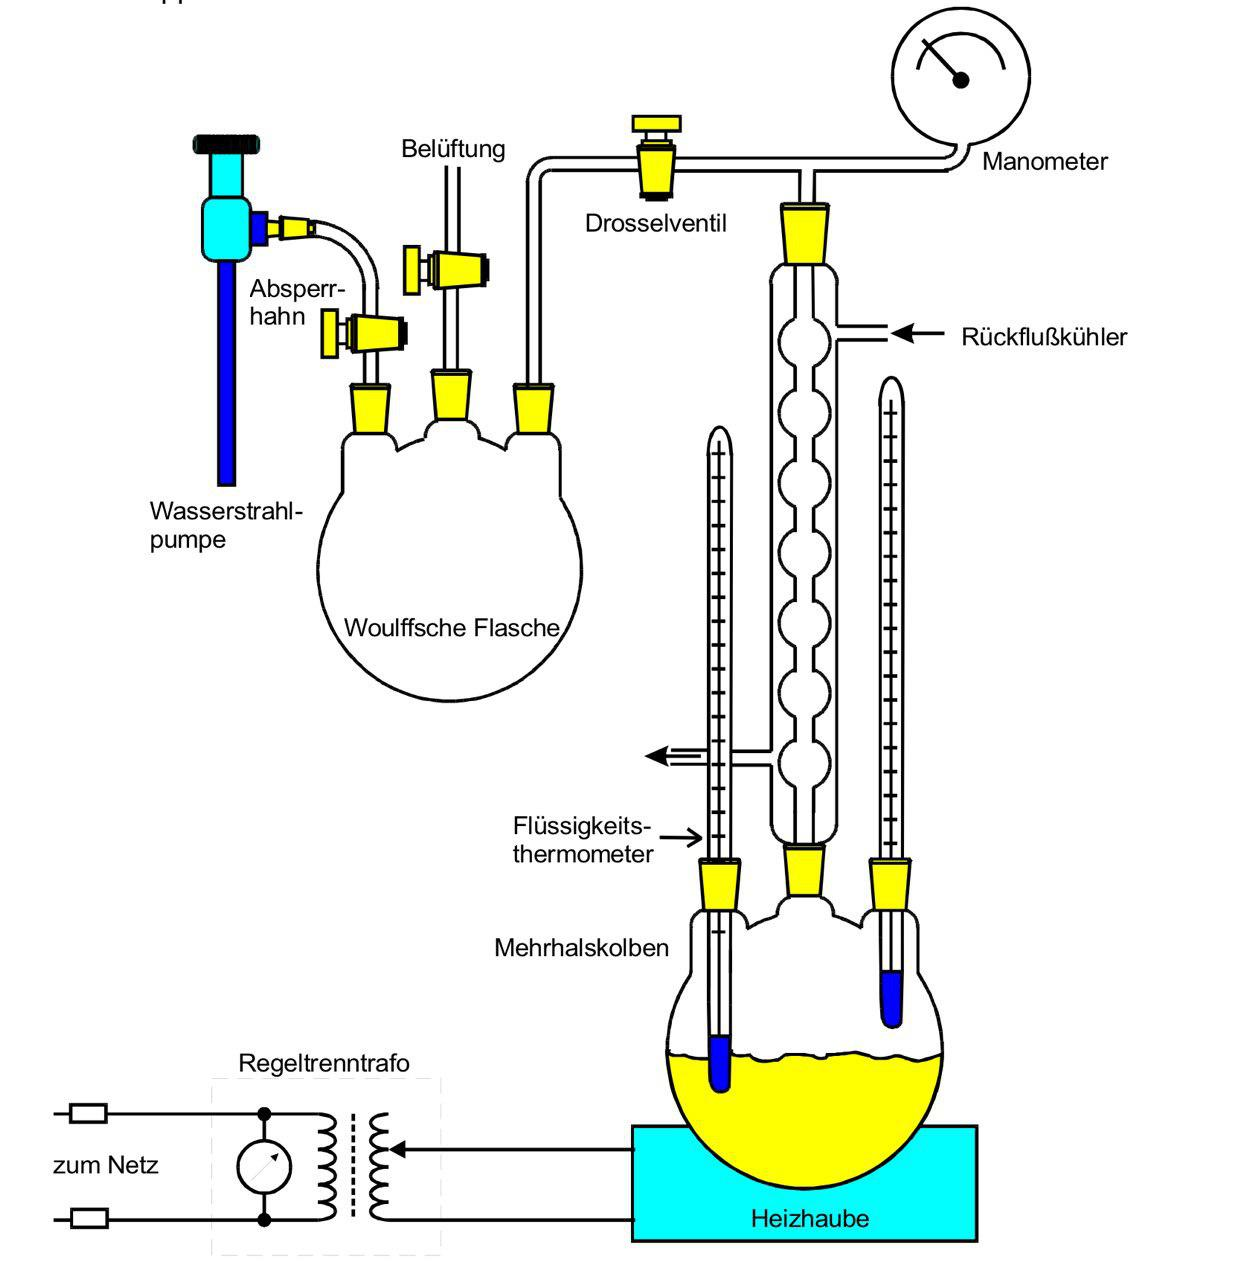
\includegraphics[width=0.7\textwidth]{bilder/anlage1.jpg}
    \caption{Apperatur 1 - niedrigdruck Bereich \cite[181]{Anleitung}}
    \label{fig:app1}
\end{figure}
Dabei wird zuerste die Apperatur mithilfe der Wasserstrahlpumpe auf
den niedrigsten Druck evakuiert (hier $p_0=26\mathrm{mbar}$).
Mithilfe der Heizhaube wir das Wasser erhitzt. Damit der aufsteigende Wasserdampf
nicht in das Manometer steigt, durchläuft den Rückfußkühler kaltes Wasser,
sodass der aufsteigende Wasserdampf wieder kondensiert.\\
Über das Flüssigkeits- und das Dampfthermometer kann die Temperatur $T$ gemessen werden.
Zur Temperaturmessung wird hier das Dampfthermometer verwendet. 
Nun wir für jedes Grad der Temperatur $T$ der passende Druck $p$ gemessen.
Wärend der Temperatursteigerung muss dabei der Rückfußkühler runter geregelt werden, bis es am
Ende nur noch tröpchenweise aus diesem läuft.\\
Die feinjustierung der Kühlung ist dabei von exentieller Wichtigkeit.
Erreicht der Dampf eine Temperatur $T \approx 95°$C so beginnt
das Kühlwasser zu sieden, Blassen zu bilden, die in der Spirale
aufzusteigen. Dies führte zu einem Druck- und Temperaturabfall.\\

Für Drücke von $p\geq 1$bar wird folgende Apperatur verwendet:
\begin{figure}
    \centering
    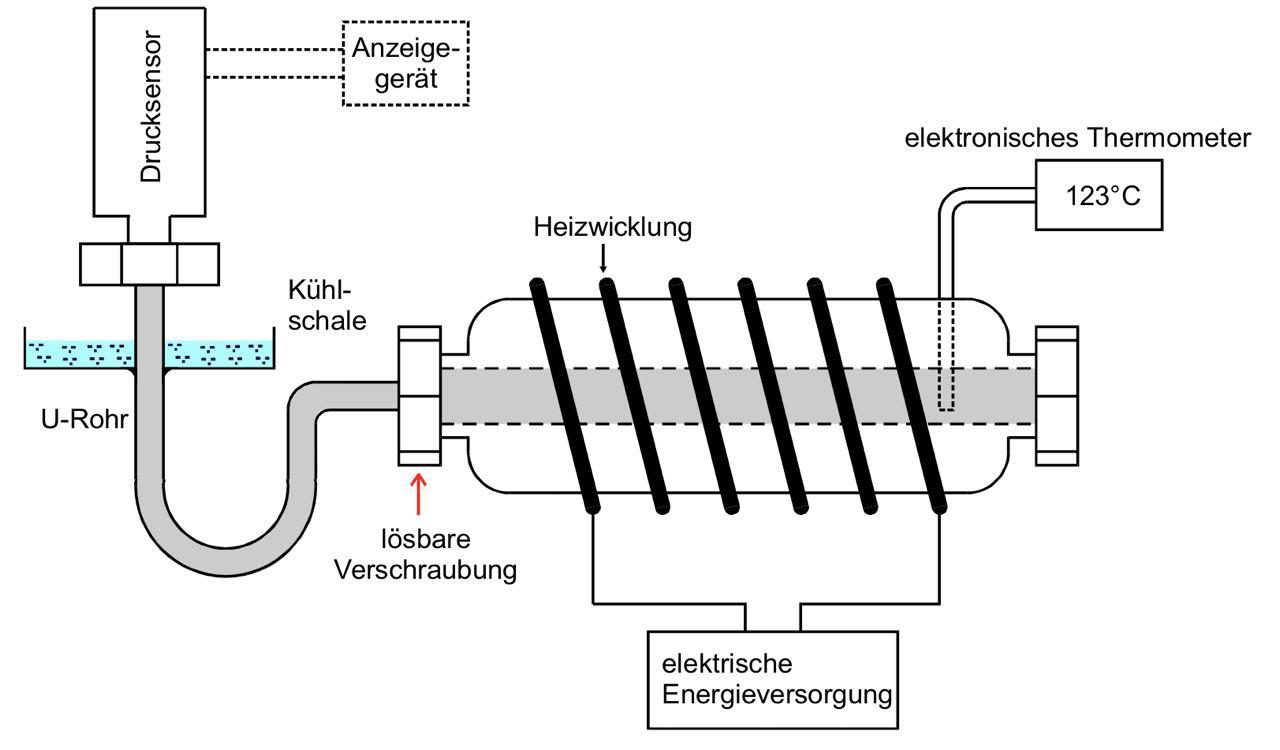
\includegraphics[width=0.7\textwidth]{bilder/analge2.jpg}
    \caption{Apperatur 2 - hochdruck Bereich \cite[183]{Anleitung}}
    \label{fig:app2}
\end{figure}

Dabei besteht der Heizkörper aus einem durchborten Stahlbolzen in dessen
Hohlraum das Wasser ist. Dieser ist von einer Heizwicklung umgeben.
Ein elektrisches Thermometer ermöglicht, die Themperatur im inneren des
Bolzens zu messen.
Auf dem Anzeigegerät kann nun der Sättigungsdruck abgelesen werden. 





%Zuerst wurde der Merhalskolben mit der Wasserstrahlpumpe evakuiert um den Druck zu minimieren.
%Nach der evakuierung wird das Wassetr im Merhalskolben erwärmt und Temperatur und Druck werden abgelesen.
